\section*{附录}
\section{图片}
\pagenumbering{roman}

\begin{figure}[H]
    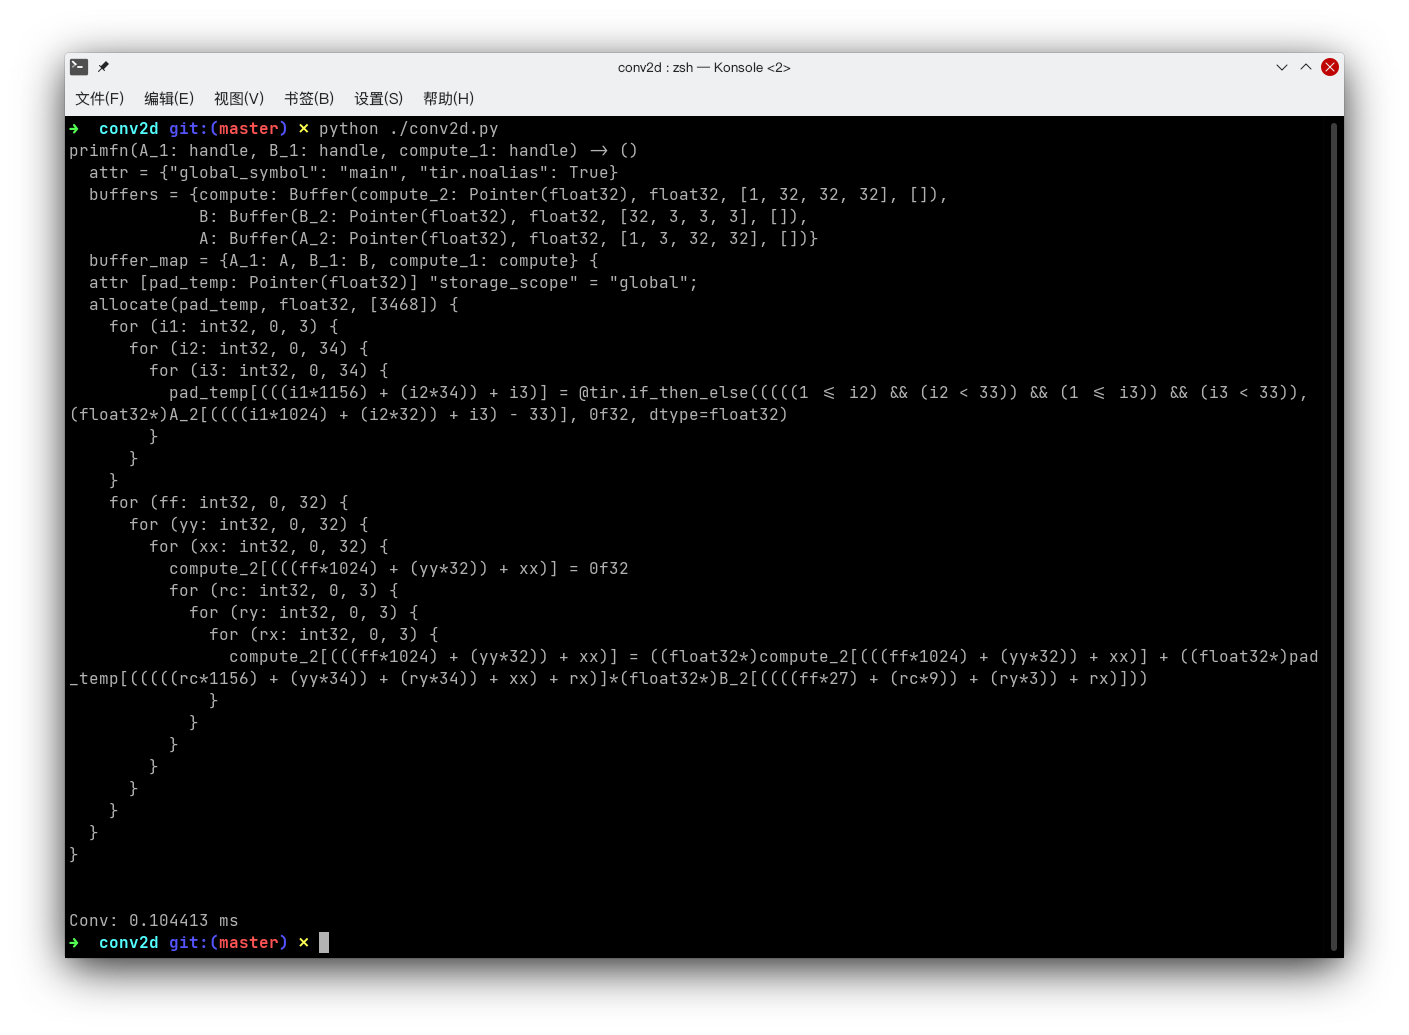
\includegraphics[width=\textwidth]{images/orig-1.png}
    \caption{小输入部分~原始计算内容}\label{1-1}
\end{figure}

\begin{figure}[H]
    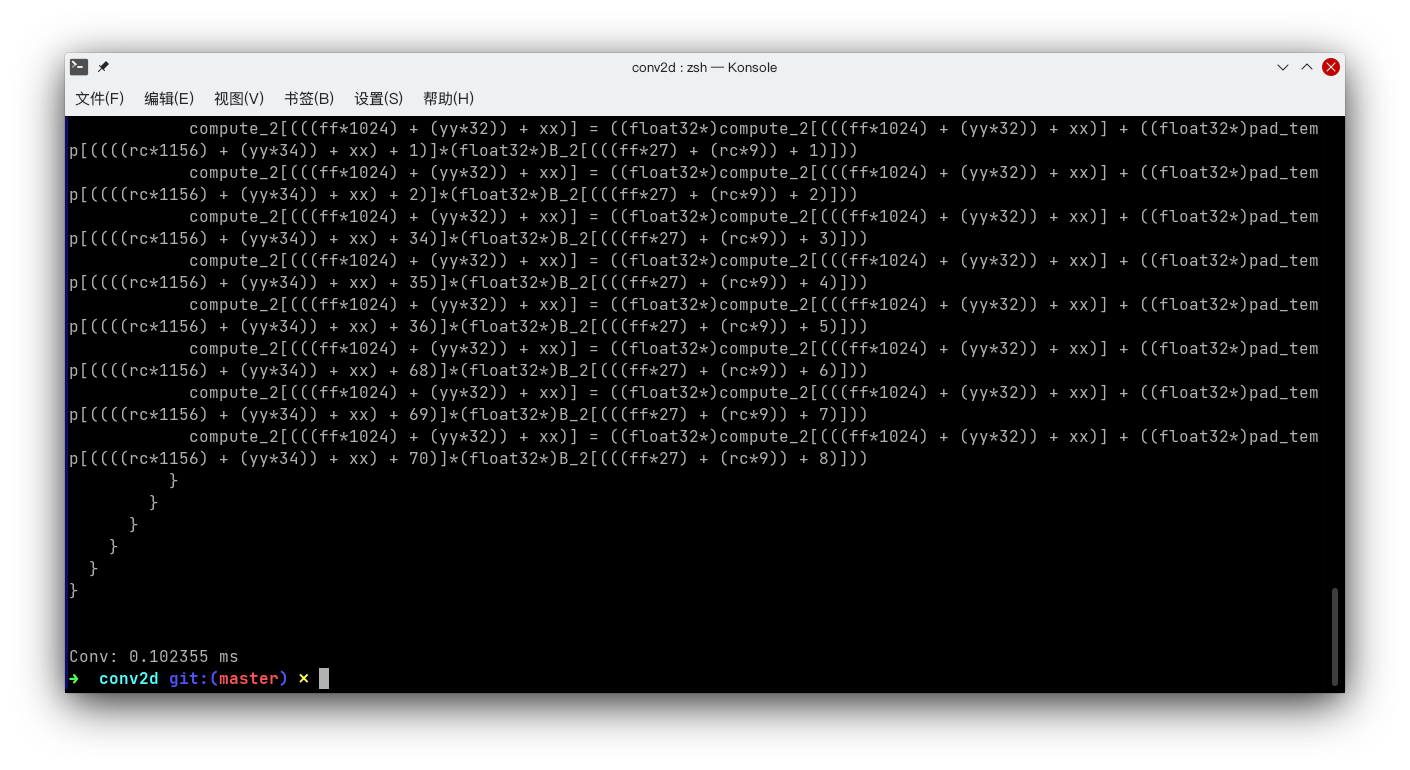
\includegraphics[width=\textwidth]{images/orig-2.png}
    \caption{小输入部分~卷积核循环展开}\label{1-2}
\end{figure}

\begin{figure}[H]
    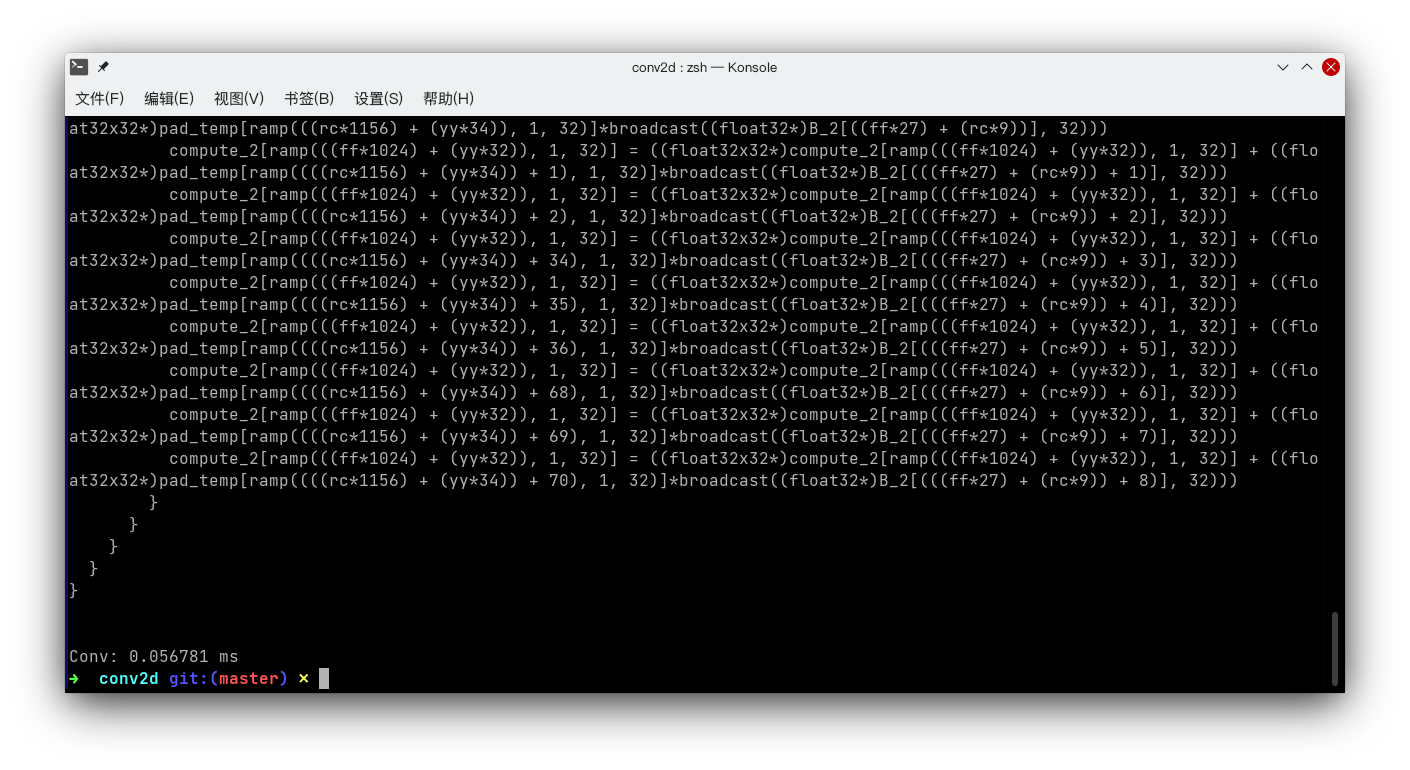
\includegraphics[width=\textwidth]{images/orig-3.png}
    \caption{小输入部分~向量化计算}\label{1-3}
\end{figure}

\begin{figure}[H]
    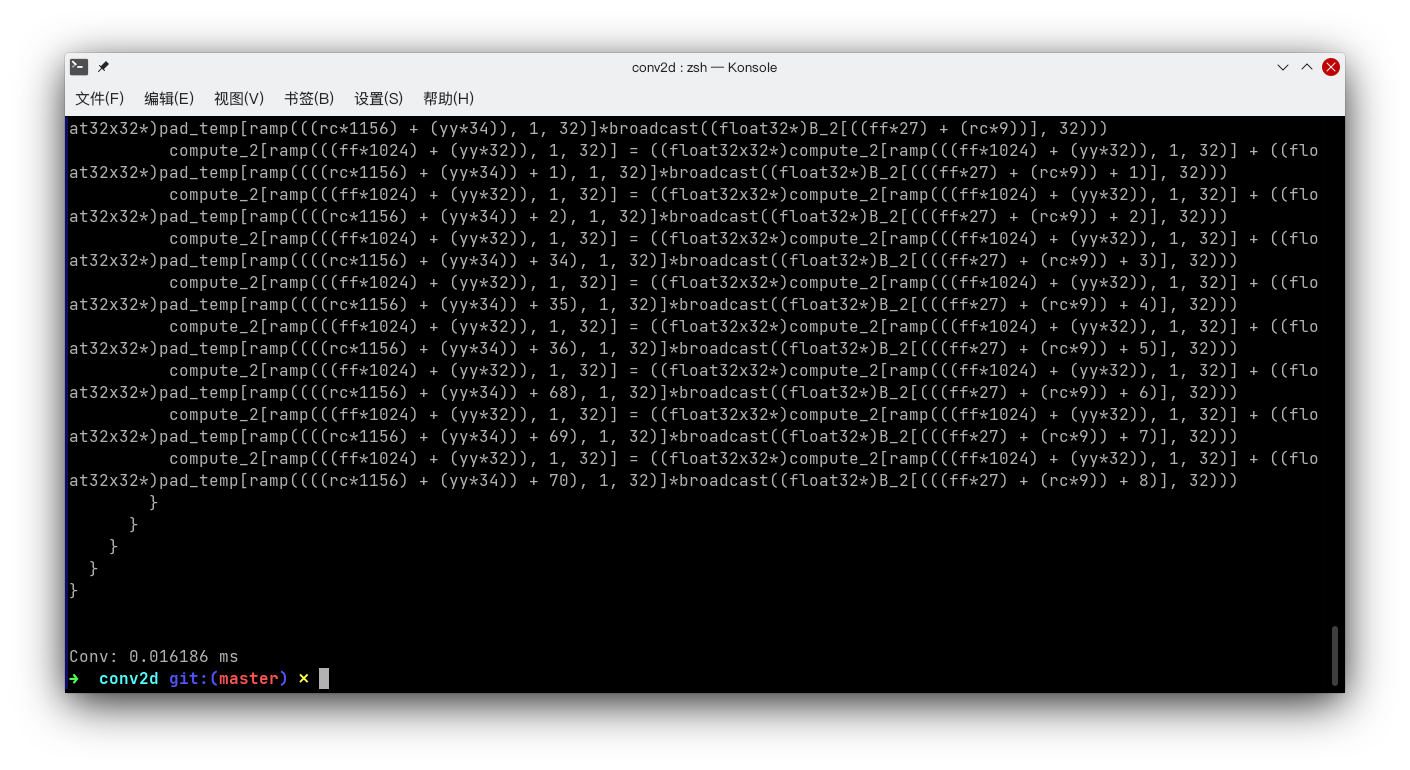
\includegraphics[width=\textwidth]{images/orig-4.png}
    \caption{小输入部分~并行执行}\label{1-4}
\end{figure}

\begin{figure}[H]
    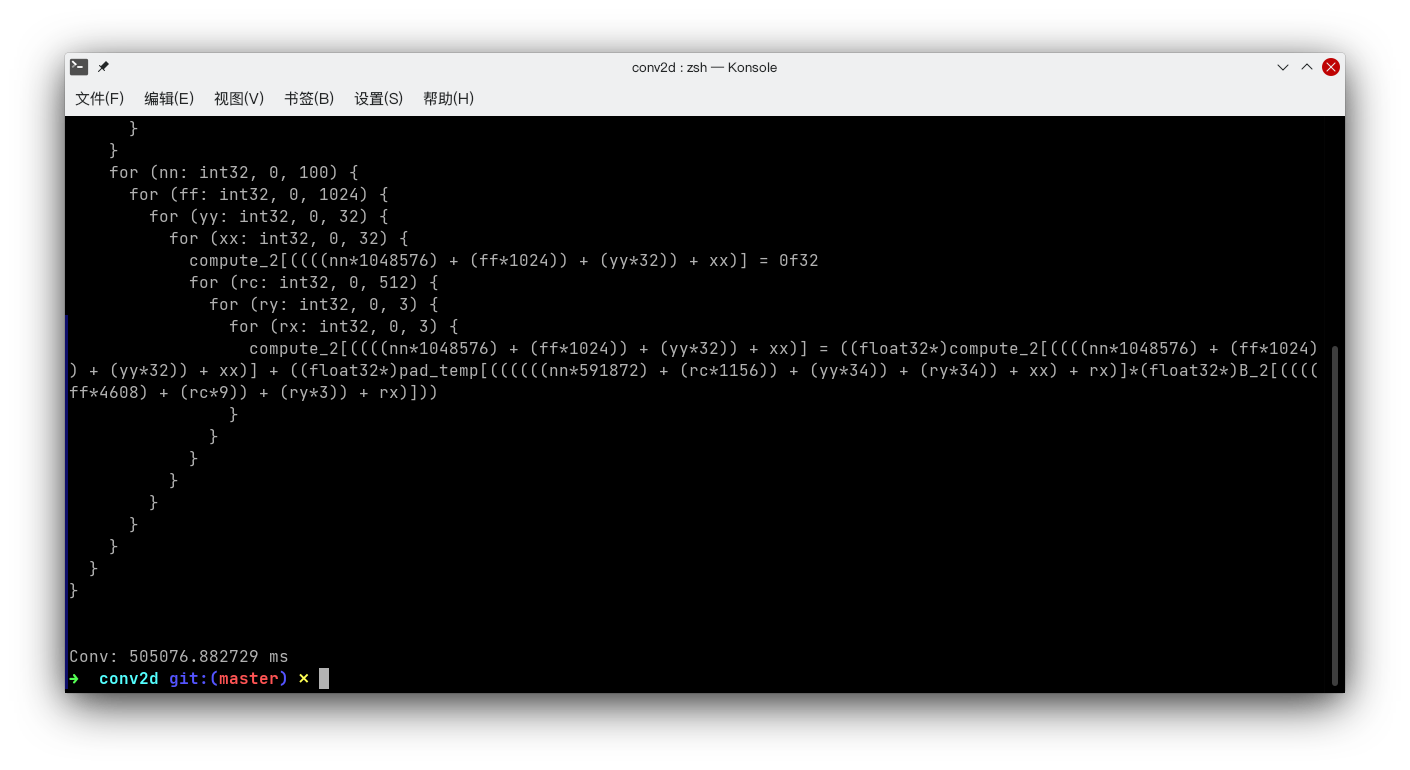
\includegraphics[width=\textwidth]{images/orig2-1.png}
    \caption{大输入部分~原始计算内容}\label{2-1}
\end{figure}
\begin{figure}[H]
    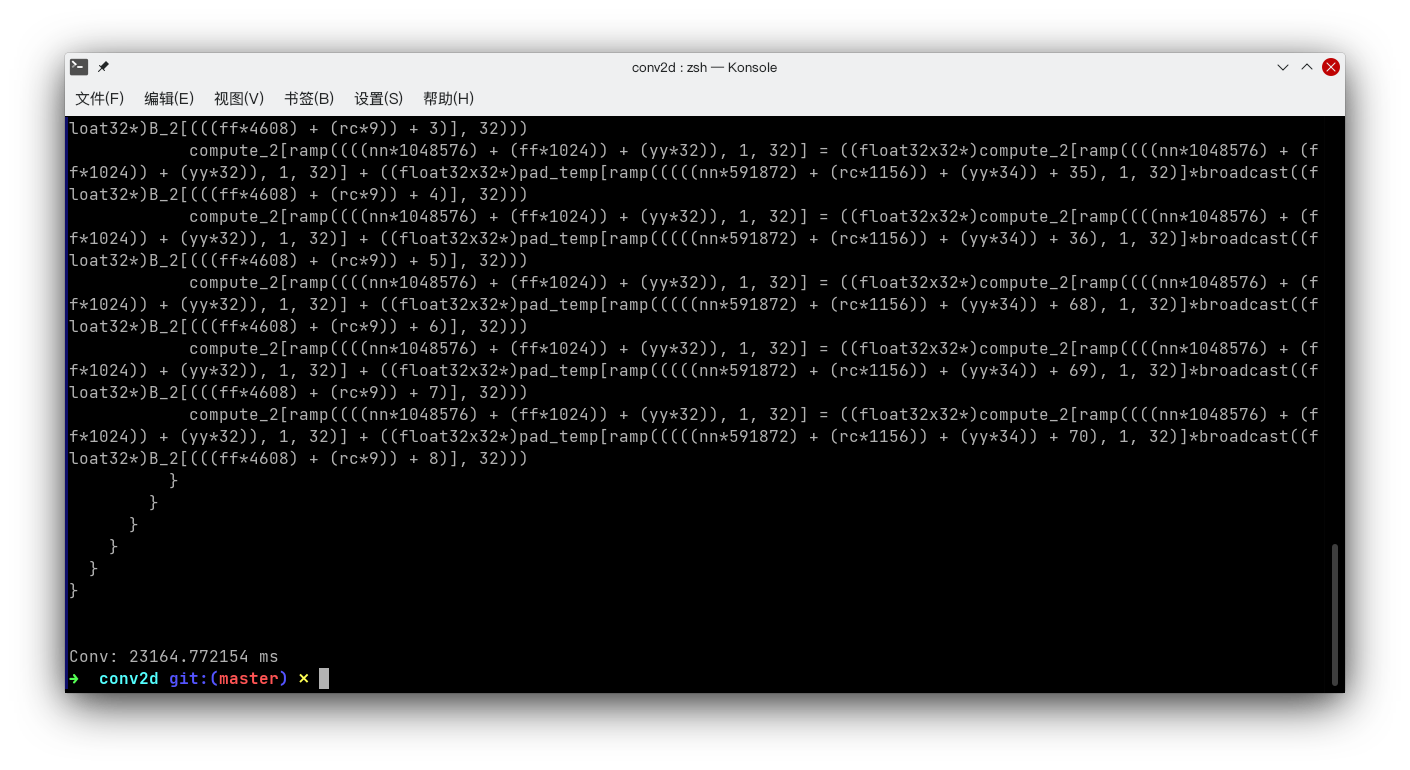
\includegraphics[width=\textwidth]{images/orig2-2.png}
    \caption{大输入部分~使用小输入优化}\label{2-2}
\end{figure}
\begin{figure}[H]
    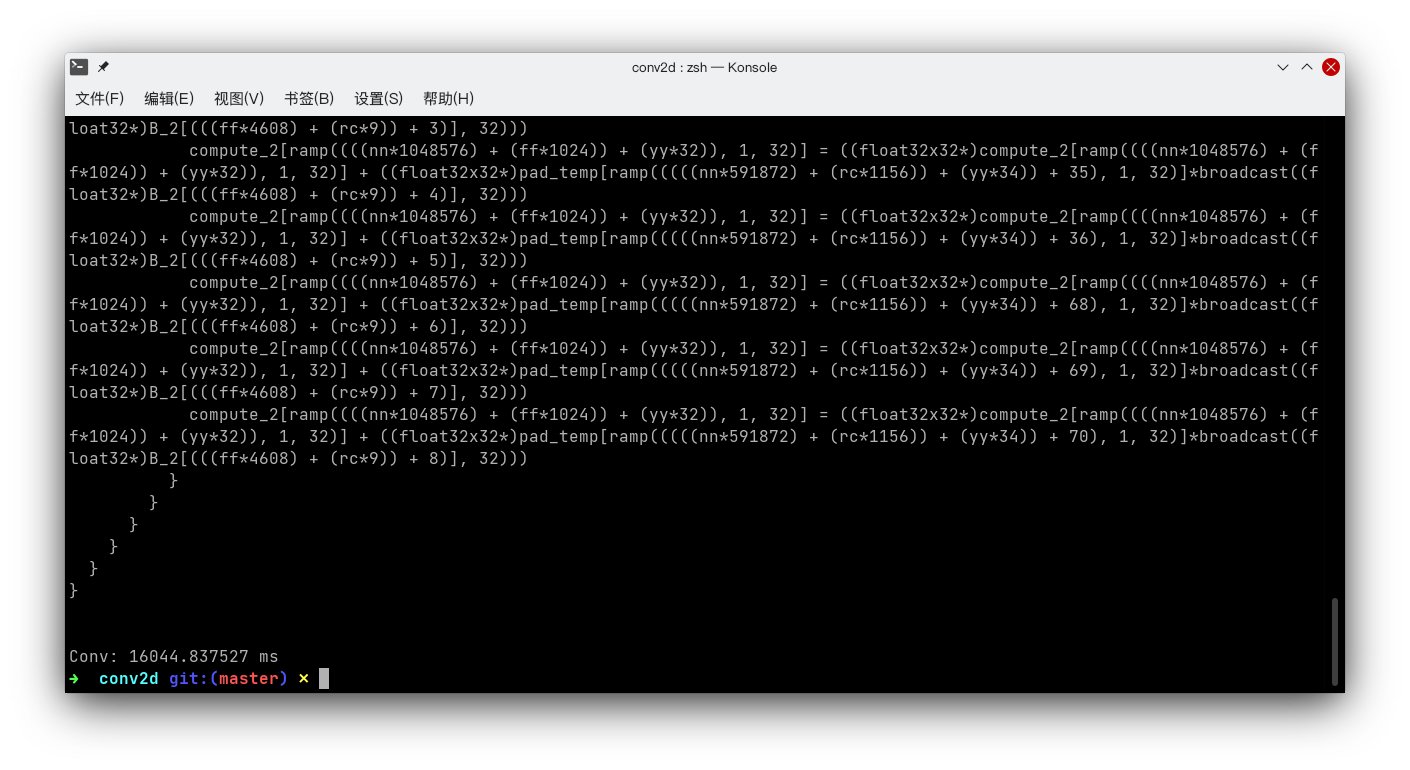
\includegraphics[width=\textwidth]{images/orig2-3.png}
    \caption{大输入部分~交换次序}\label{2-3}
\end{figure}
